Most regions of the sky are much less densely populated than M2. 
We test StarNet on run 94, camcol 1, field 12 of SDSS,
an image with light source density more typical of SDSS images.
After 10 minutes of sleep training, StarNet produced a catalog on the full $1489\times 2048$ image in $\approx2$ seconds. 
For comparison, the projected runtime of PCAT on an image of this size is 6 days.  

Since this region of the sky is more sparse, we tile the image into $50\times 50$ tiles; $N_{max}$ on tiles is three. 
Because this region of the sky also contains galaxies, only the sleep phase was employed to fit StarNet; 
the wake phase would optimize the PSF to explain both stars and galaxies. 

This image is contained in Stripe 82, a region of the sky repeatedly imaged by SDSS.
Averaging images from different runs boosts the signal to noise ratio, resulting in a ``co-added" image. 
We compare the performance of StarNet and PHOTO on the {\itshape non} co-added image. 
The PHOTO catalog of the co-added image was used as ground truth. 

The TPR of StarNet is comparable with the TPR of the PHOTO catalog on the original (non co-added) image (Figure~\ref{fig:sparse_field}). 
StarNet accrues false detections, namely galaxies, and thus we cannot compare the PPV. 
On some tiles, missed detections occur when a large galaxy within a tile causes all $N_{max}$ detections to be placed around the galaxy -- the remaining stars in the image go undetected. 
Incorporating a galaxy model would boost our performance. 


\begin{figure}[tb]
    \centering
    \begin{subfigure}{0.45\textwidth}
        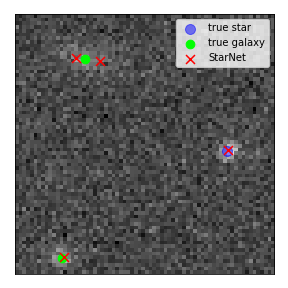
\includegraphics[width=\textwidth]{figures/sparse_field/sparse_field_detections.png}
    \end{subfigure}
    \begin{subfigure}{0.54\textwidth}
        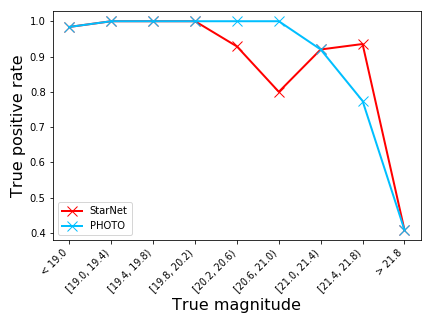
\includegraphics[width=\textwidth]{figures/sparse_field/sparse_field_tpr.png}
    \end{subfigure}
    \caption{(Left) Detections on a sparse field. 
    In this example, StarNet correctly identifies the star (blue). 
    Without a galaxy model, StarNet also classifies galaxies (green) as one or multiple stars.
    (Right) The true positive rate of StarNet and PHOTO as a function of true magnitude.}
    \label{fig:sparse_field}
\end{figure}
